\section{Evaluation} \label{sec-evaluation} 
In this section, we evaluate the performance of our proposed optimizations.

\subsection{Evaluation of Reuse and Model Warmstarting}
\subsubsection{Feature Processing Reuse}
\subsection{Model Warmstarting}
\subsection{Partial Warmstarting}

\subsection{Evaluation of Optimizing the Hyperparameter Search}
\todo[inline]{These results are still without the 'Avoiding Local Optima' solution, so ideally, once we find a good solution to avoid local optimas we should get even better results.}

In this experiment, we focus on several of the popular machine learning pipelines (flow 7707, 8353, 8315) designed for solving task 31\footnote{https://www.openml.org/t/31}, classifying customers as good or bad credit risks using the German Credit data from the UCI repository \cite{Dua:2017}.
We extracted the meta-data from the OpenML database which includes all the executions of the pipeline, the value of the hyperparameters, and the evaluation metrics.
Using the meta-data, we initialize the hyperparameter optimization process with the values of the hyperparameters for each execution and the loss ($1- accuracy$) for the specific execution.
We then execute the search with a budget of 100 trials, trying to minimize the loss of the OpenML pipelines.
We repeat this experiment 10 times, for every pipeline.
Figure \ref{fig-avg-warm-vs-cold-task-31} shows the average of losses of the 100 trials for the 10 experiments.
Warm starting the search decreases the overall loss of the trials.

\begin{figure}
\centering
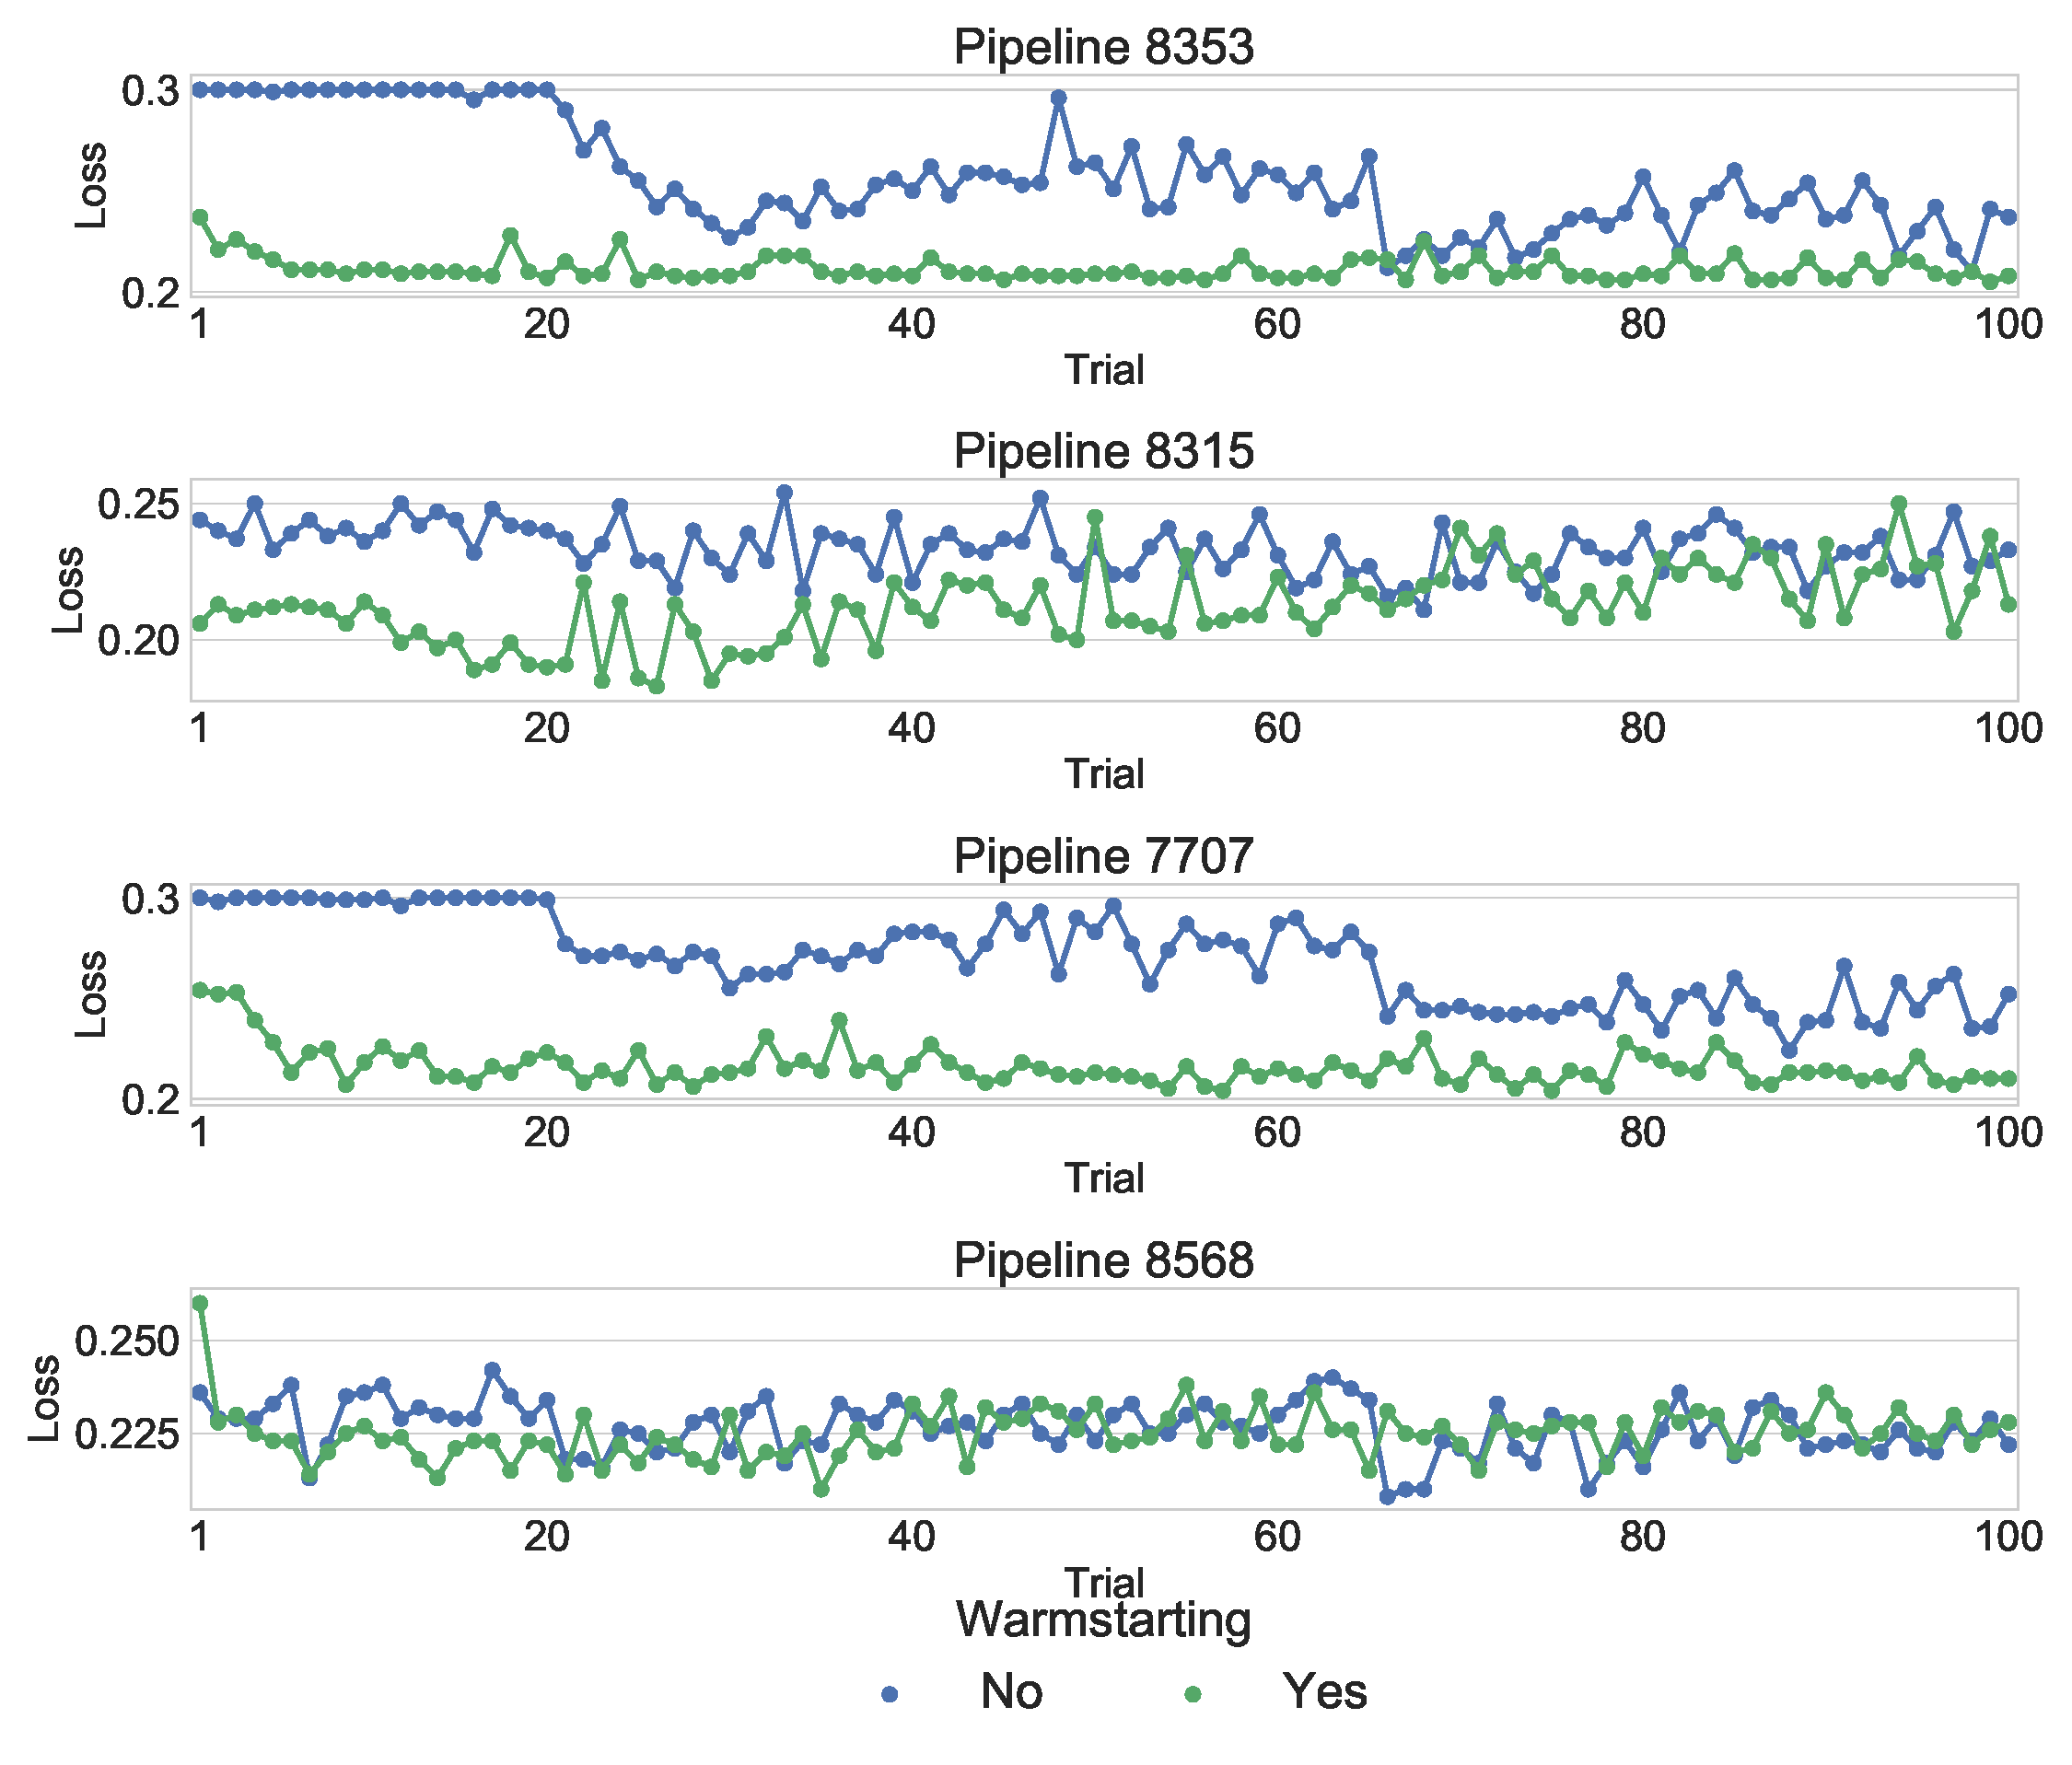
\includegraphics[width=\columnwidth]{../images/experiment-results/task31-cold-warm-trials.eps}
\caption{Loss value of 100 Trials with and without warmstarting}
\label{fig-avg-warm-vs-cold-task-31}
\end{figure}

\subsection{Avoiding Local Optima}

\subsubsection{Adaptive Selection}
In this experiment, we show the result of our adaptive selection methods on the hyperparameter search process.
Figure \ref{fig-avg-adaptive-selection-task-31} shows the result of the histogram and random selection method on the hyperparameter search process.
When compared to the vanilla approach (where full history is used in warmstarting), we see that random selection decrease the error rate of the trials where histogram increases them.
To make the difference more visible we limit the scope of the loss (y axis) from 0.20 to 0.25.
\begin{figure}
\centering
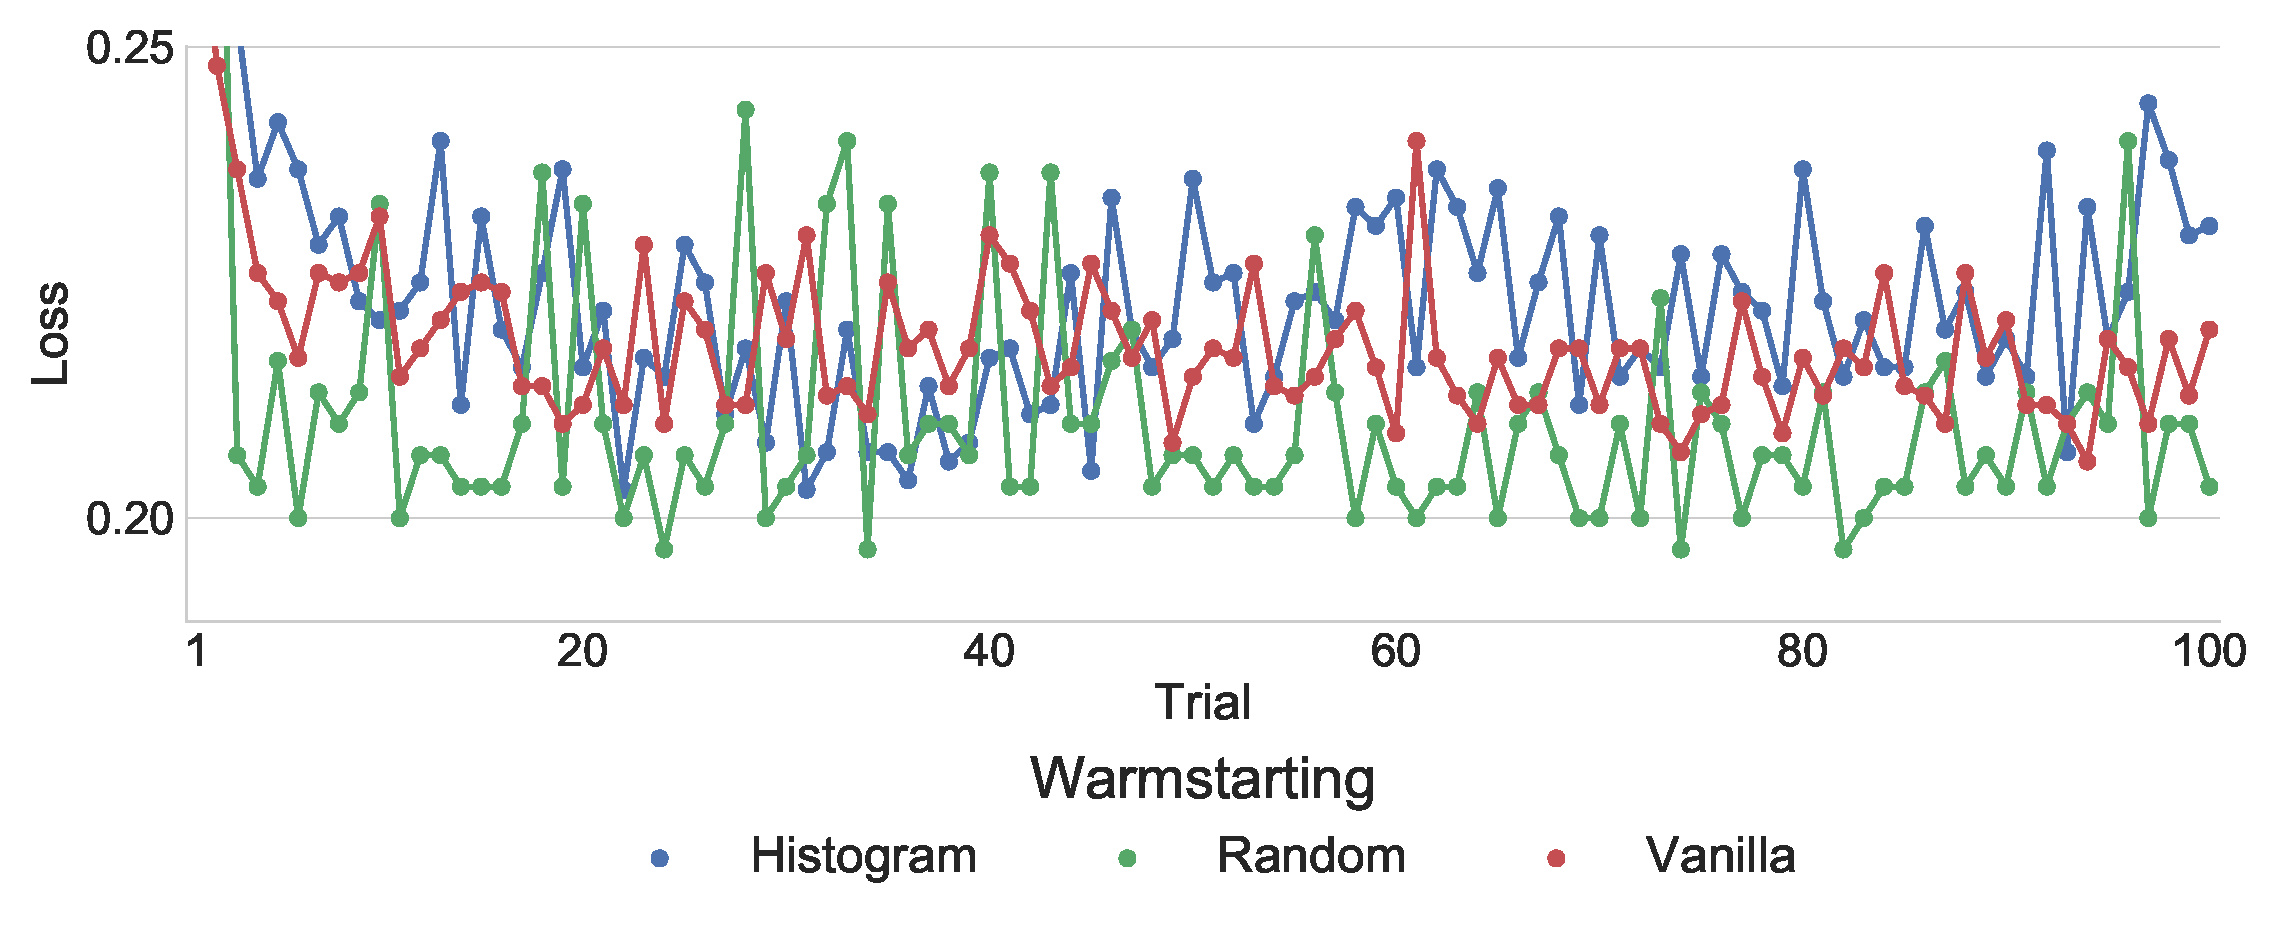
\includegraphics[width=\columnwidth]{../images/experiment-results/t31-f7707-adaptive-method-random.eps}
\caption{Effect of adaptive warmstarting on hyperparameter search process}
\label{fig-avg-adaptive-selection-task-31}
\end{figure}

\begin{table}
\centering
\begin{tabular}{crrr}
\hline
	   Pipeline & Best Loss & Warm & Cold \\ \hline
        7077 & 0.16 & 1 & 0 \\
        8315 & 0.18 & 173 & 14\\
        8353 & 0.18 &0& 1\\ 
        8568 & 0.15 &0&2\\
        \hline
\end{tabular}
\caption{Best loss and their occurrences for different pipelines using warm starting}
\end{table}

%Table \ref{table-best-hyperparameters} shows the best loss achieved from the search process for every pipeline on the Task 31.
%Figure \ref{figure-best-hyperparameters} shows the number of time that the search process (with budget of 100) manages to find the best set of hyperparameters that results in the lowest loss value.
%While both with and without warm starting does find the best set of hyperparameters, using warmstarting outperforms the search without wamrstarting and has a higher probability of finding the best hyperparameters.
%
%\begin{minipage}{\columnwidth}
%  \begin{minipage}[m]{0.49\columnwidth}
%   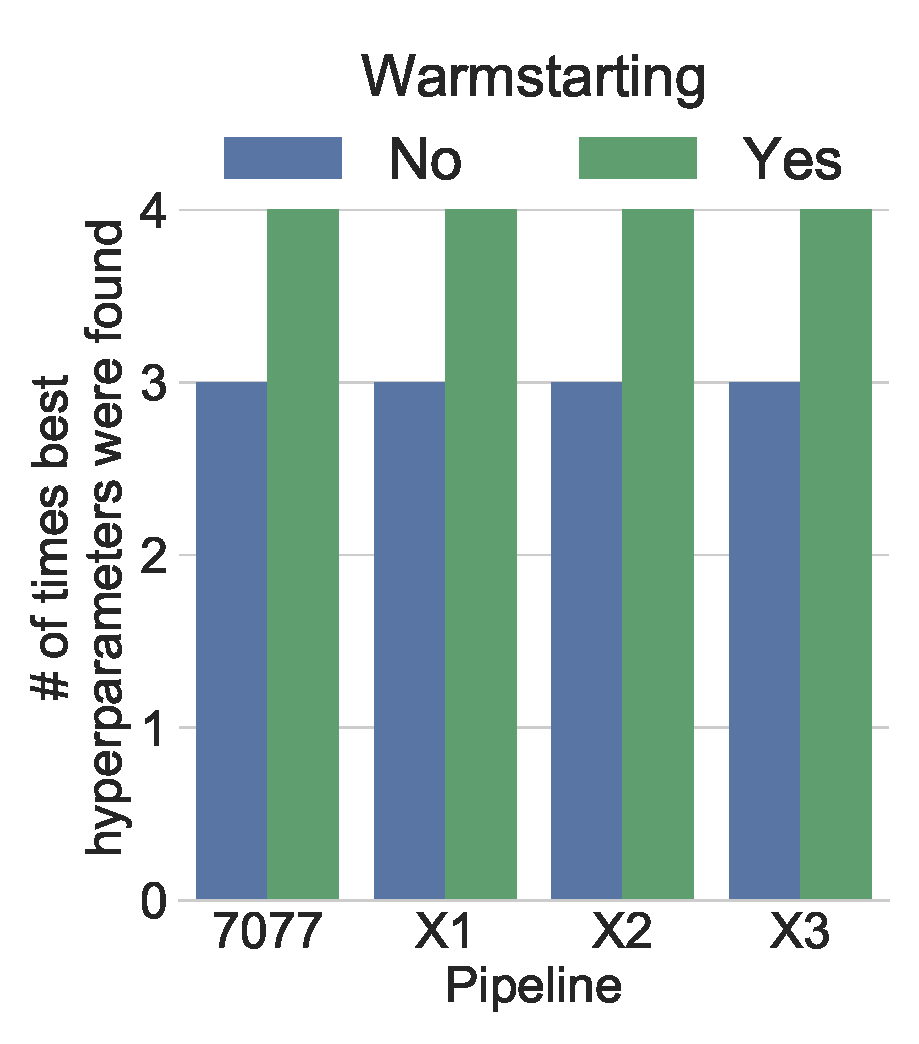
\includegraphics[width=\columnwidth]{../images/experiment-results/task31-cold-starting-warm-besthyperparametersfound.eps}
%    \captionof{figure}{Occurrences of best hyperparameters}
%     \label{figure-best-hyperparameters}
%  \end{minipage}
%  \hspace{0.5cm}
%  \begin{minipage}[m]{0.49\columnwidth}
%    \begin{tabular}{cc}\hline
%      Pipeline & Best Loss \\ \hline
%        7077 & 0.189 \\
%        X1 & XXX \\
%        X2 & XXX \\ \hline
%      \end{tabular}
%      \captionof{table}{Best hyperparameters}
%      \label{table-best-hyperparameters}
%    \end{minipage}
%  \end{minipage}
%\subsection{Data Materialization}